\section{Clase 22}
\subsection{Expansión instantánea y paradoja de Gibbs}
Considere la siguiente situación
\begin{figure}[h!]
	\centering
	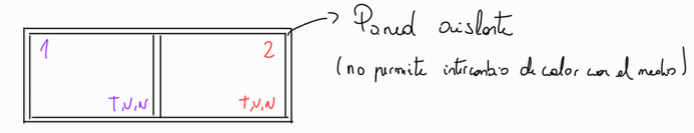
\includegraphics[scale=0.3]{fig/22-img.png}
\end{figure}
Los compartimiento $1$ y $2$ tienen el mismo volúmen, y cada comportamiento contiene moleculas contiene moléculas de un tipo de gas ideal (ideal, monoatómico, sin spin) diferente. Las moléculas de cada tipo de gas son indistinguibles, pero las moléculas de gases diferentes se pueden diferenciar.

Sea $T_1,P_1,\m_1$ y $T_2,P_2,\m_2$  las temperaturas, presiones y potenciales químicos 
%TODO seguir ejercicio





\subsection{Correcciones cuánticas del teorema de equipartición}
\subsubsection{Excitaciones moleculares}
Consideremos $N$ sistemas cuánticos, cada uno de los cuales tiene niveles de energía $l$ con degenerancia $g_l$ y energía $\epsilon_l$.

La función partición canónica de cada sistema está dada por
\begin{equation}
\boxed{  Z_{\rm int}=\sum_lg_le^{-\epsilon_l/\k T}}
\end{equation}
donde int indica que es una función partición sobre grados de libertad internos.

Luego, la energía promedio por sistema está dada por
\begin{equation}
  \ev{\frac{E_{\rm int}}{N}}=-\pdv{\b}\ln(Z_{\rm int	})=\frac{\sum_lg_l\epsilon_le^{-\epsilon_l/\k T}}{Z_{\rm int}}
\end{equation}

\begin{ej} \textbf{Oscilador armónico}
	
	Para el oscilador armónico se tiene que
	\begin{align}
  g_l&=1\\
  \epsilon_l&=\hbar\omega(l+1/2)
\end{align}
Ahora para onstruir la función partición, hay que sustraer la energía del vacío. La razón es que $T\to 0$, solo el estado de vacío puede estar ocupado.
\end{ej}
